% Generated shared reviewed material.
\section{Hubs, spokes and the topology retained by a dessin}
\label{hs:section}
The hubs-and-spokes construction in the HoTT book, Sections~6.6--6.8
\cite{HubsSpokes}, gives a useful language for attaching cells. For a loop
$f:S^1\to X$, form the homotopy pushout
$X\cup_f CS^1$: add a fresh hub and paths from every $f(u)$ to that hub,
continuously indexed by $u:S^1$. This attaches a disk, rather than merely a
finite graph of radial edges. The book's Remark~6.7.1 explains why identifying
the hub with an existing boundary point requires extra coherence;
Remark~6.7.2 distinguishes propositional from judgmental computation.

For our dessins the useful distinction is geometric. A vertex star has a
disk neighborhood with a specified cyclic ordering of its incident bands.
Removing the disk center gives a punctured disk, which retains its peripheral
loop. Removing only the vertex of a finite star instead leaves disconnected
open rays. These operations cannot be interchanged. In a cellular dessin,
filling a face imposes its attaching-word relation; leaving its center
punctured retains a boundary component of the ribbon neighborhood.

\begin{center}
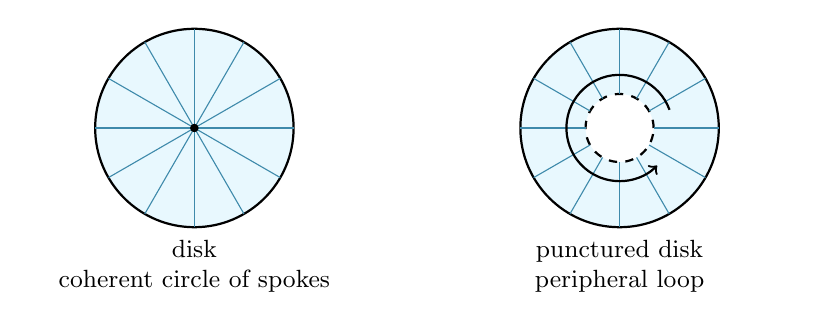
\begin{tikzpicture}[scale=.9]
 \fill[cyan!9] (0,0) circle (1.4);
 \draw[thick] (0,0) circle (1.4);
 \foreach \a in {0,30,...,330}{\draw[cyan!65!black] (0,0)--(\a:1.4);}
 \fill (0,0) circle (.06);
 \node[align=center,text width=4cm,font=\small] at (0,-1.95) {disk\\coherent circle of spokes};
 \begin{scope}[xshift=6cm]
  \fill[cyan!9,even odd rule] (0,0) circle (1.4) (0,0) circle (.48);
  \draw[thick] (0,0) circle (1.4);
  \draw[dashed,thick] (0,0) circle (.48);
  \foreach \a in {0,30,...,330}{\draw[cyan!65!black] (\a:.48)--(\a:1.4);}
  \draw[->,thick] (20:.75) arc (20:315:.75);
  \node[align=center,text width=4cm,font=\small] at (0,-1.95) {punctured disk\\peripheral loop};
 \end{scope}
\end{tikzpicture}
\end{center}
The shaded regions are two-dimensional; the displayed finite spokes sample
them. The annulus shown on the right is a deformation retract of the punctured
disk, not a missing vertex in a one-dimensional graph.

\begin{proposition}[Face filling changes the covering problem]
Let a connected cellular dessin be a spine of an oriented genus-$g$ ribbon
surface with $n>0$ boundary components. Its graph fundamental group is free
of rank $2g+n-1$. Capping all boundary components gives the presentation
\[
 \left\langle a_1,b_1,\ldots,a_g,b_g\ \middle|\
       \prod_{i=1}^g[a_i,b_i]=1\right\rangle.
\]
For the one-face clean dessins $K_{2,3}$ and $K_{2,5}$ used here, these free
ranks are respectively $2$ and $4$, before capping.
\end{proposition}
\begin{proof}
A spanning-tree collapse of the connected spine leaves $E-V+1$ circles.
The ribbon surface retracts onto that spine and has Euler characteristic
$2-2g-n=V-E$, proving the rank formula. Cutting a surface along a standard
system of handle arcs gives the boundary word
$\prod_i[a_i,b_i]\prod_jc_j$. Van Kampen therefore presents its group by
these generators and this one relation. With a boundary present, eliminate
$c_n$, leaving the stated free group. Capping attaches disks along the $c_j$,
so van Kampen sets each $c_j=1$, giving the closed-surface presentation.
For our rotations on $K_{2,m}$, both black vertices have the same cyclic
order on the $m$ incident edges. Suppressing the bivalent white vertices
gives dart rotations $(0\,\cdots\,m-1)(m\,\cdots\,2m-1)$ and involution
$i\leftrightarrow i+m$. The face permutation is one $2m$-cycle for odd $m$.
Thus $V=m+2$, $E=2m$, $F=1$, and $g=(m-1)/2$, giving both examples.
\end{proof}

The once-punctured torus and closed torus both have $H_1\cong\mathbb Z^2$,
but their groups are $F_2$ and $\mathbb Z^2$; only the closed torus has
$H_2\cong\mathbb Z$. The analogous genus-two groups are $F_4$ and the
four-generator surface group, with $H_1\cong\mathbb Z^4$ in both cases.
Indeed the standard closed-surface cellular complex has one vertex,
$2g$ edges and one face. The face word is a product of commutators, so its
abelianized boundary is zero. Removing the face leaves the wedge of circles.
This computes the stated homology and also explains why $H_1$ alone misses
the face relation. The torus group is abelian while $F_2$ is not; in higher
genus the closed surface has nonzero $H_2$ while the graph does not.

Consequently the graph's universal cover is a tree, whereas the universal
cover of the filled genus-two surface includes lifted faces and is a disk.
Collapsing a spanning tree changes the combinatorial cover graph; the Cayley
tree of a free basis is not literally the original biregular dessin cover.
This distinction matters when lifting strings, periodic paths and boundary
conditions in the infinite locally gentle algebra.

The gluing language organizes local patches and their compatibility maps.
It does not reconstruct the ribbon cyclic order, complex structure, Belyi
map, quadratic zero relations, coefficient ring or polynomial/formal/operator
completion from the homotopy type alone. These data are retained explicitly
in the existing dessin and order constructions. Descent of modules, derived
categories, Hom-control, AR meshes or Fukaya categories needs a separately
defined functor and hypotheses; a homotopy pushout of underlying spaces is
not such a theorem. Nor does it imply an arithmetic determinant identity.

The accompanying tool computes the same one-face genus-one/two/four dart
families and draws local disk/annulus patches and their surface polygon
presentations, peripheral loops and face words. These
are exact finite combinatorial checks plus the topological proof above.
HoTT is referenced as a conceptual foundation; no univalence or higher
inductive-type axiom is added to the pinned Lean4 development. Its complete
cell-attachment and categorical formalization remains an explicit task.
